% 5-page core narrative — expand for journal; use PLOS template at submission.
\documentclass[10pt,twocolumn]{article}
\usepackage[margin=2cm]{geometry}
\usepackage{graphicx}
\usepackage{booktabs}
\usepackage{amsmath}
\usepackage{hyperref}
\usepackage{subcaption}
\usepackage{xcolor}
\newcommand{\todo}[1]{\textcolor{red}{[TODO: #1]}}

\title{Decoder-only conditional latent models with temporal mixture priors for unsupervised cross-lab mouse sleep staging and substage discovery}
\author{Oliver Rosb\ae{}k Elmgreen \and Morten M\o{}rup \and Birgitte Rahbek Kornum}
\date{}

\begin{document}
\maketitle

\begin{abstract}
Manual mouse sleep scoring lacks cross-lab consensus, and supervised deep models generalize poorly across acquisition sites until retrained on multi-laboratory labels \cite{rose2026consensus}.
We address this with unsupervised population learning on the Mouse Sleep Staging Validation dataset (MSSV) and a controlled model ladder: feature-domain HMM, HMM--GMVAE, decoder-only cGMVAE, and decoder-only cHMM--GMVAE with a warm sticky HMM--GMM latent prior.
On joint cross-lab holdout (leave-mice-out cv4fold), cHMM--GMVAE reaches best-of-three prior NMI up to $0.65$ (fold~4), versus $0.28$--$0.41$ for matched cGMVAE and $0.51$ for the MSc thesis HMM feature baseline.
Holdout staging uses \emph{zero-shot} inference---encoding without subject identifiers and assigning states from the temporal mixture prior only---in contrast to transductive tools such as AccuSleep that require per-mouse manual calibration \cite{barger2019accusleep}.
A substage resolution sweep and physiology panels refine Wake/NREM/REM structure and transition substages \cite{katsageorgiou2018mcRBM}.
\end{abstract}

\section{Introduction}
Rodent sleep is scored from EEG and EMG into Wake, NREM, and REM, yet montage and lab protocols differ \cite{rose2025mssv}.
Rose et al.\ show that manual scoring lacks cross-lab consensus and that published deep models generalize poorly across MSSV sites until retrained on multi-laboratory data \cite{rose2026consensus}---motivating label-agnostic staging and rigorous holdout evaluation.
Supervised models such as SPINDLE and REST achieve high cross-lab accuracy but require expert labels \cite{miladinovic2019spindle,wang2026rest}.
Unsupervised tools include classical FASTER clustering \cite{sunagawa2013faster}, FASTER2 Gaussian HMMs on hand-crafted features \cite{yamada2024faster2}, SegWay's per-mouse k-means plus HMM smoothing \cite{yaghouby2016segway}, mcRBM substage discovery \cite{katsageorgiou2018mcRBM}, and recent WUCSS light/deep NREM states \cite{cusinato2024wucss}; none combine deep latent learning, sticky mixture priors, and population zero-shot holdout on MSSV.

Our MSc thesis showed that subject-conditioned GMVAEs improve population staging ($\mathrm{NMI}\approx 0.70$) over feature HMMs ($\approx 0.51$) \cite{elmgreen2026thesis}, with interpretable substages but encoder conditioning that leaks subject identity at evaluation.
\textbf{Contributions:} (i)~decoder-only cVAE conditioning with \textbf{zero-shot holdout inference} (no subject embeddings at staging); (ii)~temporal HMM--GMM prior (cHMM--GMVAE) in a fair ladder against cGMVAE and HMMGMVAE; (iii)~substage biology with expert validation.
Thesis synthetic validation, encoder+decoder ablations, and full $K{=}13$ taxonomy are in Supplementary Material.

\section{Methods}
\textbf{Data.} MSSV (OpenNeuro ds006366): labs 2, 3, 5; 4\,s epochs; expert Wake/NREM/REM labels for evaluation only \cite{rose2025mssv}.
\textbf{Features.} Per-lab spectral front-end locks (\texttt{cvae\_overrides}); wide MLP encoder--decoder, latent dimension 6 \cite{elmgreen2026thesis}.
\textbf{Models.} Ladder: HMM on features (thesis); HMMGMVAE ($\mathit{emb}{=}0$, $T{=}64$, \texttt{hmm\_gmm}); cGMVAE (decoder-only, $\mathit{emb}{=}8$, GMM prior); cHMM--GMVAE (+ warm sticky HMM--GMM, $\kappa{=}0.92$) \cite{dilokthanakul2016gmvae,sohn2015cvae,ebbers2017hmmvae,johnson2016svae}.
\textbf{Training.} Population training on cv4fold training mice (joint: all labs; within-lab: single lab). Subject embeddings ($\mathit{emb}{=}8$) are concatenated to the decoder only (\texttt{decoder\_only\_conditioning}), not the encoder, during reconstruction and prior learning.
\textbf{Inference (holdout).} For held-out validation mice, sleep-state labels are obtained by encoding spectral epochs \textbf{without subject identifiers}, then assigning states via the learned Gaussian mixture or sticky HMM--GMM prior on latent means (prior prediction). Subject embeddings are \textbf{not} used at holdout evaluation; the decoder is not invoked for staging. This is zero-shot with respect to subject identity and contrasts with AccuSleep-style mixture z-scoring that requires $\sim$10\,min of manually scored baseline data per new mouse \cite{barger2019accusleep}.
\textbf{Evaluation.} Leave-mice-out cv4fold holdout; prior-prediction NMI vs expert macro labels; best of three seeds.
\textbf{Substages.} Sweep $K\in\{3,5,7,9,11,13,15\}$ mixture components; physiology grid and transition matrix \cite{katsageorgiou2018mcRBM,grieger2021prerem}.

\section{Results}
\subsection{Cross-lab holdout ladder}
Figure~\ref{fig:ladder} summarises joint-scope holdout NMI (\todo{refresh when all 12 locked jobs finish}).
On completed folds, cHMM--GMVAE exceeds cGMVAE by $+0.11$ to $+0.35$ NMI (joint mean: $0.55$ vs.\ $0.33$, $n{=}3$--$4$ folds).
Within-lab holdout shows lab heterogeneity: cHMM leads on lab~3 (up to $0.746$), while cGMVAE remains competitive on lab~2 (Supplementary Table~S1).

\begin{figure}[t]
  \centering
  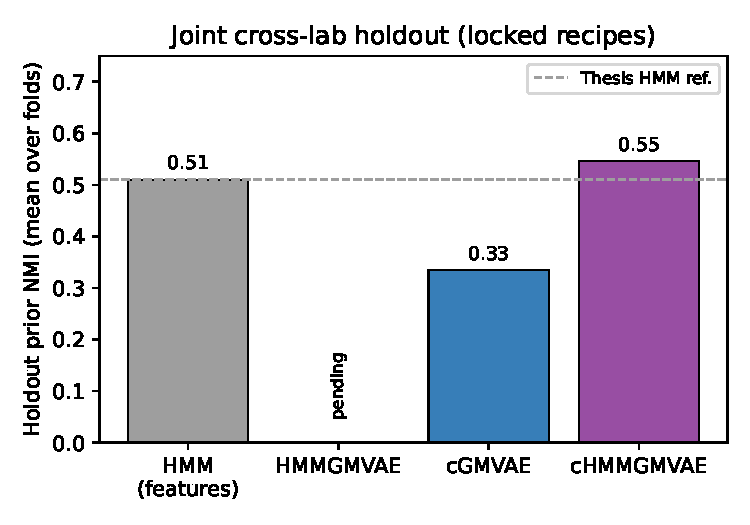
\includegraphics[width=\linewidth]{figures/figure2_ladder.pdf}
  \caption{\textbf{Model ladder on joint holdout.} Bars: best-of-three prior NMI per fold. Dashed line: thesis HMM feature baseline ($0.51$).}
  \label{fig:ladder}
\end{figure}

\begin{table}[t]
  \centering
  \caption{Joint holdout prior NMI (best-of-three per fold, locked recipes).}
  \label{tab:joint}
  \small
  \begin{tabular}{lccc}
    \toprule
    Fold & HMM$^\dagger$ & cGMVAE & cHMM--GMVAE \\
    \midrule
    1 & 0.51 & 0.361 & 0.612 \\
    2 & 0.51 & 0.275 & 0.381 \\
    3 & 0.51 & 0.407 & \todo{run} \\
    4 & 0.51 & 0.296 & 0.646 \\
    \bottomrule
  \end{tabular}
  \\[0.5em]
  {\footnotesize $^\dagger$Thesis population LOSO reference, not re-estimated per fold.}
\end{table}

\subsection{Substages and transitions}
Figure~\ref{fig:substage} shows a compact physiology panel (placeholder from decoder-only cGMVAE; \todo{replace with cHMM $K$-sweep winner}).
Rare/confounded states are excluded after expert review (see Interview Guide).
Transition substages concentrate at macro boundaries \cite{grieger2021prerem}; transition matrix and hypnogram in Figure~\ref{fig:transition}.

\begin{figure*}[t]
  \centering
  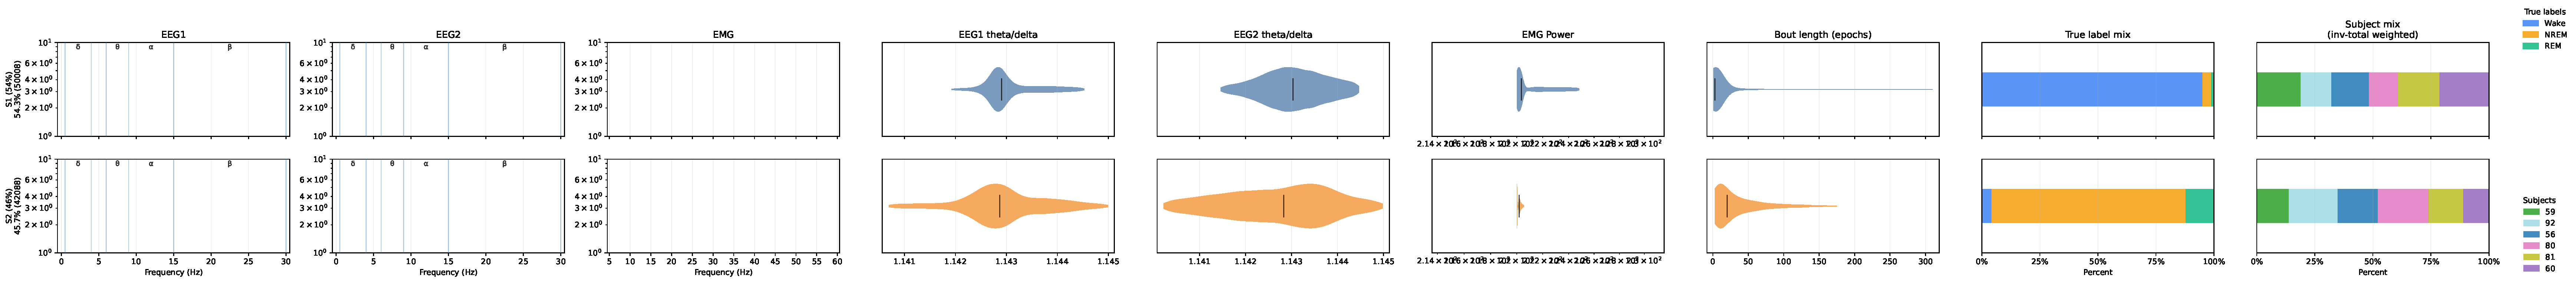
\includegraphics[width=0.95\textwidth]{figures/figure3_substage_panels.pdf}
  \caption{\textbf{Substage physiology.} Rows: discovered substates; columns: EEG/EMG PSD, $\theta/\delta$, EMG power, bout length, macro-label mix, subject mix.}
  \label{fig:substage}
\end{figure*}

\begin{figure}[t]
  \centering
  \begin{subfigure}{\linewidth}
    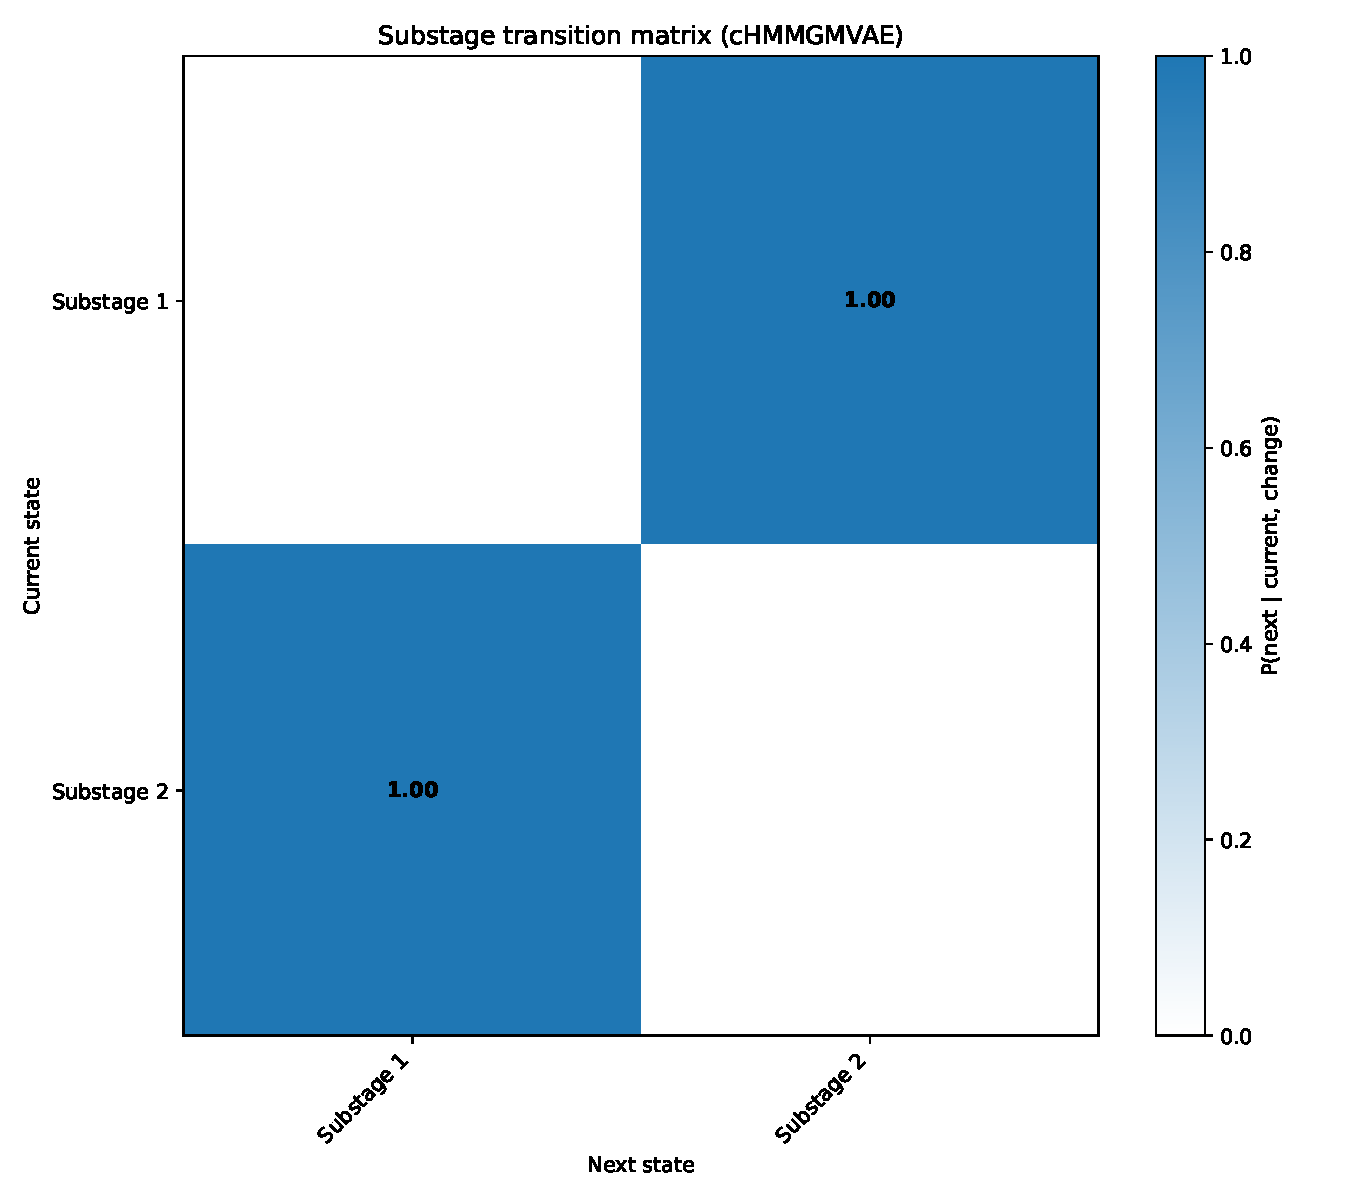
\includegraphics[width=\linewidth]{figures/figure4_transition_matrix.pdf}
  \end{subfigure}
  \begin{subfigure}{\linewidth}
    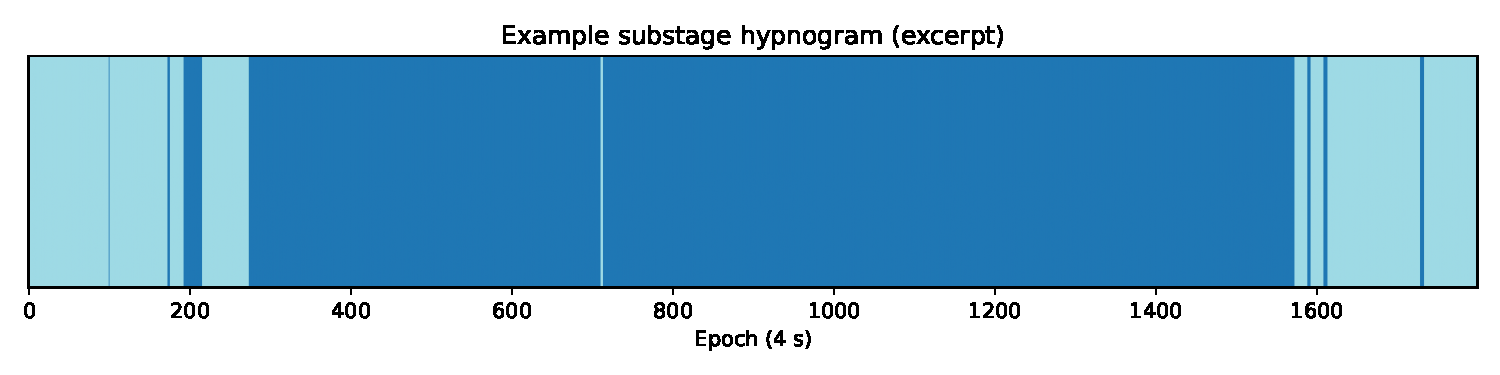
\includegraphics[width=\linewidth]{figures/figure4_hypnogram_excerpt.pdf}
  \end{subfigure}
  \caption{Substage transition matrix and example hypnogram excerpt.}
  \label{fig:transition}
\end{figure}

\section{Discussion}
Rose et al.\ establish that cross-lab supervised staging inherits rater disagreement \cite{rose2026consensus}; our unsupervised ladder complements this by discovering structure without training on one lab's label biases.
Zero-shot holdout inference (encoder + temporal prior, no subject ID) contrasts with transductive calibration in AccuSleep and per-animal fitting in SegWay \cite{barger2019accusleep,yaghouby2016segway}.
Temporal mixture priors help when bout structure and lab-specific spectra align with sequence modelling (lab~3/5); static GMM decoders suffice on some montages (lab~2).
Decoder-only conditioning is the main methodological advance over the thesis encoder--decoder setup for population holdout.
Absolute holdout NMI remains below curated thesis LOSO; relative gains over the ladder and substage biology are the primary claims.
Limitations: seed fragility, per-lab preprocessing locks (not per-mouse manual scoring), and pending HMMGMVAE locked runs.
Expert naming of active-awake and transition substates (Kornum lab) grounds biological interpretation versus mcRBM \cite{katsageorgiou2018mcRBM}.

\section*{Code availability}
SPA repository: locked recipes, config generators, postprocess, and figure scripts (\texttt{docs/paper/}).

\bibliographystyle{plain}
\bibliography{references}

\end{document}
